%%%%%%%%%%%%%%%%%%%%%%%%%%%%%%%%%%%%%%%%%%%%%%%%%%%%%%%%%%%%%%%%%%%%%%
% Lớp 10 | Hàm số bậc hai và đồ thị | Hàm số bậc hai
% Dạng 0D3?2-1: Xác định hàm số bậc hai
% Số câu: 40  (sinh tự động bởi tach_cau.py; từ nay thầy sửa trực tiếp file này)
%%%%%%%%%%%%%%%%%%%%%%%%%%%%%%%%%%%%%%%%%%%%%%%%%%%%%%%%%%%%%%%%%%%%%%

%%%%%%%%%%%%%%%% TRẮC NGHIỆM 4 PHƯƠNG ÁN %%%%%%%%%%%%%%%%

% nguồn: MaHoaNH_TracNghiem_Lop10
\begin{ex}%[0D3N2-1]%[ma:c3499347]
	Cho  parabol có phương trình $y=x^2-2x+3$. Trục đối xứng của đồ thị hàm số là đường thẳng
	\choice 
		 {$x=3$}
		 {$x=-2$}
		{\True  $x=1$}
		{$x=\dfrac{3}{2}$} 
	\loigiai{Trục đối  xứng $x=\dfrac{-b}{2a}=\dfrac{-(-2)}{2\cdot1}=1$.}
\end{ex}

% nguồn: MaHoaNH_TracNghiem_Lop10
\begin{ex}%[0D3N2-1]%[ma:b7c34531]
	Parabol $\left(P\right)\colon y=2x^2-4x+3$ có trục đối xứng là  đường thẳng có phương trình là
	 \choice
		{$x=2$} 
		{$x=-1$} 
		 {\True $x=1$}
		 {$x=-2$}
	 \loigiai{
	Ta  có $a=2$, $b=-4$, (P) có trục đối xứng là đường thẳng có phương trình $x=-\dfrac{b}{2a}=1$.}
\end{ex}

% nguồn: MaHoaNH_TracNghiem_Lop10
\begin{ex}%[0D3N2-1]%[ma:26e66995]
	Tọa độ đỉnh $S$ của parabol $\left(P\right)\colon  y=-3x^2+2x+1$ là
	 \choice
		 {$S\left( -\dfrac{2}{3}; -\dfrac{5}{3} \right)$}
		 {$S\left( \dfrac{2}{3}; 1 \right)$}
		{\True $S\left( \dfrac{1}{3}; \dfrac{4}{3}  \right)$}
		{$S\left(  -\dfrac{1}{3}; 0 \right)$}
	 \loigiai{
		Parabol có tọa độ đỉnh là $S\left( -\dfrac{b}{2a}; -\dfrac{\Delta }{4a} \right)\Rightarrow S\left( \dfrac{1}{3};  \dfrac{4}{3} \right)$.
	} 
\end{ex}

% nguồn: MaHoaNH_TracNghiem_Lop10
\begin{ex}%[0D3N2-1]%[ma:09c35be4]
	Cho hàm số $y=x^2-2x-3$. Khẳng định nào sau đây là  đúng?
	\choice 
		{Đồ thị hàm số là một đường  thẳng}
		{\True Đồ thị hàm  số là một Parabol}
		{Hàm số đồng biến trên $\mathbb{R}$} 
		{Hàm  số nghịch biến trên $\mathbb{R}$}
	\loigiai{ 
		Do hàm số $y=x^2-2x-3$ là  hàm số bậc hai nên đồ thị hàm số là một Parabol.
	 }
\end{ex}

% nguồn: MaHoaNH_TracNghiem_Lop10
\begin{ex}%[0D3N2-1]%[ma:a8b5253a]
	Trục đối xứng của  parabol $(P)\colon y=2x^2+6x+3$ là
	\choice 
		 {\True $x=-\dfrac{3}{2}$}
		 {$x=-\dfrac{2}{3}$}
		{$x=-3$} 
		{$y=-3$} 
	 \loigiai{
		Trục  đối xứng $x=-\dfrac{b}{2a}=-\dfrac{6}{2\cdot2}=-\dfrac{3}{2}$.
	 }
\end{ex}

% nguồn: MaHoaNH_TracNghiem_Lop10
\begin{ex}%[0D3N2-1]%[ma:8cd4bfaf]
	Hàm số nào dưới đây là  hàm số bậc hai?
	 \choice
		 {$y=x^4+3x^2+2$}
		{$y=\dfrac{1}{x}$} 
		{$y=x+1$} 
		{\True $y=x^2+2$} 
	 \loigiai{
		Hàm số bậc  hai là $y=x^2+2$.
	} 
\end{ex}

% nguồn: MaHoaNH_TracNghiem_Lop10
\begin{ex}%[0D3N2-1]%[ma:05982543]
	Trong các biểu  thức sau, biểu thức nào là tam thức bậc 2?
	 \choice
		{\True $f_1(x)  = 15x^2 - 10$}
		{$f_2(x) = \sqrt{6x^2 + 15x  - 10}$}
		{$f_3(x)  = 15x - 10 + \dfrac{1}{x^2}$}
		{$f_4(x)  = 6x + 9$}
	 \loigiai{
		Tam thức  bậc hai có dạng tổng quát là $ ax^2 + bx + c $ với $ a \neq 0 $.\\
		Vậy đáp án  đúng là $ f_1(x) = 15x^2 - 10 $.
	 }
\end{ex}

% nguồn: MaHoaNH_TracNghiem_Lop10
\begin{ex}%[0D3N2-1]%[ma:5bb14943]
	\immini[thm]{Hàm  số nào sau đây có đồ thị như hình dưới đây?
	\choice 
		 {$y=x^2-3x+1$}
		{$y=-x^2+3x-1$} 
		{$y=-2x^2+3x-1$} 
		{\True$y=2x^2-3x+1$} 
		} 
		{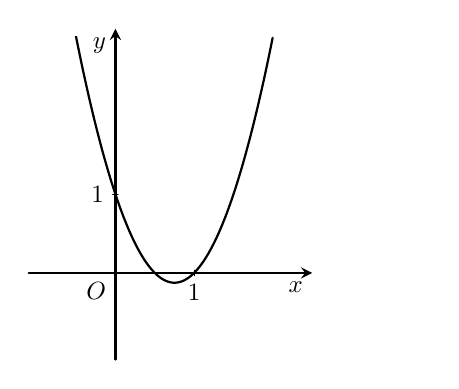
\begin{tikzpicture}[line join=round,line cap=round,>=stealth,thick]
		\tikzset{every  node/.style={scale=0.9}}
		 \draw[->] (-1.1,0)--(2.5,0) node[below left] {$x$};
		\draw[->] (0,-1.1)--(0,3.1)  node[below left] {$y$};
		\draw (0,0) node [below  left] {$O$};
		\foreach \x/\nx in {1/1} 
		 \draw[thin] (\x,1pt)--(\x,-1pt) node [below] {$\nx$};
		 \foreach \y/\ny in {1/1}
		 \draw[thin] (1pt,\y)--(-1pt,\y) node [left] {$\ny$};
		\begin{scope}
			\clip (-1,-1)  rectangle (4,3);
			\draw[samples=200,domain=-1:2,smooth,variable=\x] plot (\x,{2*(\x)^2+-3*(\x)+1}); 
		\end{scope}
	\end{tikzpicture}
		} 
	 \loigiai{
		Bề lõm  của parabol hướng lên trên suy ra $a>0$.\\
		Suy ra  loại đáp án $y=-x^2+3x-1$ và $y=-2x^2+3x-1$.\\
		Đồ thị đi qua điểm $(1; 0)$ nên  chọn $y=2x^2-3x+1$.
	} 
\end{ex}

% nguồn: MaHoaNH_TracNghiem_Lop10
\begin{ex}%[0D3H2-1]%[ma:8b8a3975]
	Parabol $y=ax^2+bx+1$ đi qua hai điểm $A(1;4)$ và  $B(-2;7)$ có phương trình là
	\choice 
		{$ y=x^2+x+1$} 
		{$  y=2x^2+2x$}
		{$ y=2x^2+2x+1$} 
		{\True $ y=2x^2+x+1$} 
	\loigiai{Thay toạ độ điểm $A(1;4)$ và  $B(-2;7)$ vào $y=ax^2+bx+1$ ta có $$\heva{&a+b=3\\&4a-2b=6}\Leftrightarrow\heva{&a+b=3\\&4a-2b=6}\Leftrightarrow\heva{&a=2\\&b=1.}$$
	 Vậy $ y=2x^2+x+1$.}
\end{ex}

% nguồn: MaHoaNH_TracNghiem_Lop10
\begin{ex}%[0D3H2-1]%[ma:a66a25cb]
	Xác định parabol  $(P)\colon y=2x^2+bx+c$, biết $(P)$ qua điểm $M(0;4)$ và có trục đối xứng $x=1$.
	\choice 
		 {\True $y=2x^2-4x+4$}
		{$y=2x^2+4x-3$} 
		 {$y=2x^2-3x+4$}
		 {$y=2x^2+x+4$}
	 \loigiai{
		Từ giả thiết ta có hệ phương trình $\heva{&4=c\\&\dfrac{-b}{4}=1}\Leftrightarrow\heva{&b=-4\\&c=4}\Rightarrow(P)\colon  y=2x^2-4x+4$.
	 }
\end{ex}

% nguồn: MaHoaNH_TracNghiem_Lop10
\begin{ex}%[0D3H2-1]%[ma:a0e9f2f7]
	Tọa độ đỉnh của  parabol $y=-3x^2+6x-1$ là
	\choice 
		{$ I(-1;-10) $} 
		{$ I(2;-1)  $}
		 {\True $ I(1;2) $}
		{$ I(-2;-25) $} 
	 \loigiai{
		Tọa độ đỉnh của parabol $y=ax^2+bx+c$ $(a\neq 0)$ là $I\left(-\dfrac{b}{2a};-\dfrac{b^2-4ac}{4a}\right)$ nên tọa độ đỉnh của parabol đã cho  là $I(1;2)$.
	} 
\end{ex}

% nguồn: MaHoaNH_TracNghiem_Lop10
\begin{ex}%[0D3H2-1]%[ma:2c950d59]
	 Hàm số $y=-x^2+2x-5$ đồng biến trên khoảng
	\choice 
		 {$(-\infty;-1)$}
		 {$(-1;+\infty)$}
		{\True $(-\infty;1)$} 
		{$(1;+\infty)$} 
	\loigiai{ 
		Vì hàm số $y=-x^2+2x-5$ là hàm số bậc hai có $a=-1 < 0$ và hoành độ đỉnh $-\dfrac{b}{2a}=1$  nên hàm số đồng biến trên $(-\infty;1)$.
	} 
\end{ex}

% nguồn: MaHoaNH_TracNghiem_Lop10
\begin{ex}%[0D3H2-1]%[ma:6ef4cd30]
	Cho parabol $y=a x^2+b x+4$ có trục đối xứng là đường thẳng $x=\dfrac{1}{3}$ và đi qua điểm $A(1; 3)$. Tổng giá  trị $a+2 b$ là
	 \choice
		{$-\dfrac{1}{2}$} 
		 {$\dfrac{1}{2}$}
		{$-1$} 
		 {\True $1$}
	 \loigiai{
		Ta có $\heva{&-\dfrac{b}{2 a}=\dfrac{1}{3}\\&A(1; 3) \in(P)}\Leftrightarrow \heva{&2 a+3  b=0\\&a+b+4=3}\Leftrightarrow\heva{&2 a+3 b=0\\&a+b=-1}\Leftrightarrow\heva{&a=-3\\&b=2.}$\\
		Vậy  $a+2 b=-3+2 \cdot 2=1$.
	} 
\end{ex}

% nguồn: MaHoaNH_TracNghiem_Lop10
\begin{ex}%[0D3H2-1]%[ma:e7a43304]
	Biết Parabol $y=ax^2+bx-4$ có  đỉnh $I(-1;-5)$. Tìm $a$ và $b$.
	 \choice
		 {$a=1;b=-2$}
		{\True$a=1;b=2$} 
		{$a=0;b=-3$} 
		 {$a=-1;b=2$}
	 \loigiai{
		Ta có $(P)$ nhận đường thẳng $x=-1$ làm  trục đối xứng nên $-\dfrac{b}{2a}=-1\Rightarrow b=2 a$.\\
		$(P)$  đi qua điểm $I(-1;-5)$ nên $a-b-4=-5 \Rightarrow a-b=-1$.\\
		Giải hệ phương  trình $\heva{&b=2a\\&a-b=-1}\Leftrightarrow\heva{&a=1\\&b=2.}$
	} 
\end{ex}

% nguồn: MaHoaNH_TracNghiem_Lop10
\begin{ex}%[0D3H2-1]%[ma:e63d3b28]
	Cho Parabol  $P \colon y=x^2+mx+n$ ($m,\,n$ tham số). Xác định $m,\,n$ để $(P)$ nhận đỉnh $I\left(2;\,-1\right)$ .
	\choice 
		{\True  $m=-4,\,n=3$}
		 {$m=4,\,n=3$}
		 {$m=4,\,n=-3$}
		 {$m=-4,\,n=-3$}
	 \loigiai{
		Parabol $(P)\colon y=x^2+mx+n$ nhận $I\left(2;-1\right)$ là đỉnh,  khi đó ta có
		\[\heva{&4+2m+n=-1\\&-\dfrac{m}{2}=2} 
		\Leftrightarrow \heva{&2m+n=-5\\&m=-4} 
		\Leftrightarrow \heva{&n=3\\&m=-4.}\] 
	 Vậy $m=-4,\,n=3$ .}
\end{ex}

% nguồn: MaHoaNH_TracNghiem_Lop10
\begin{ex}%[0D3H2-1]%[ma:0321fbc9]
	\immini{Đường parabol trong hình vẽ bên có  thể là đồ thị của hàm số nào trong các hàm số sau
	 \choice
		 {$y=-x^2+2x-2$}
		 {\True $y=x^2-2x-2$}
		{$y=x^2+2x-2$} 
		 {$y=-x^2-2x-2$}
		}{ 
		\begin{tikzpicture}[line join=round,line cap=round,font=\footnotesize,scale=0.7,>=stealth]
				 \draw[-stealth](-1.5,0)--(4,0) node[above]{$x$};
				 \draw[-stealth](0,-3.3)--(0,2) node[right]{$y$};
				 \draw[smooth,samples=100,domain=-1.1:3.1] plot (\x,{(\x)^2-2*\x-2)});
				\fill (0,0)  circle (1pt) node[above left]{$O$};
			\end{tikzpicture}
		 }
	\loigiai{ 
		Dựa vào đồ thị ta thấy Parabol có $a>0$, hoành  độ đỉnh $x=-\dfrac{b}{2a}>0$.\\
		Nên hàm số $y=x^2-2x-2$ có đồ thị phù hợp với hình  vẽ.
	} 
\end{ex}

% nguồn: MaHoaNH_TracNghiem_Lop10
\begin{ex}%[0D3Y2-1]%[ma:58b9c20c]
	Trong các biểu thức dưới đây, biểu thức nào là  một tam thức bậc hai?
	 \choice
		{\True $f(x)=x^2+3$} 
		{$f(x)=0 x^2+2  x$}
		{$f(x)=\dfrac{1}{x^2}$} 
		{$f(x)=2 x+1$} 
	 \loigiai{
		Trong các biểu thức trên, $f(x)=x^2+3$ là một  tam thức bậc hai.
	} 
\end{ex}

% nguồn: MaHoaNH_TracNghiem_Lop10
\begin{ex}%[0D3B2-1]%[ma:7ce74e57]
	Toạ  độ đỉnh $I$ của parabol $(P)\colon y=x^2+2x+4$ là
	\choice 
		{$I(2;5)$} 
		{\True $I(-1;3)$} 
		{$I(-1;1)$} 
		 {$I(1;7)$}
	\loigiai{ 
		Toạ độ đỉnh  $I$ là $\heva{&x_I=\dfrac{-b}{2a}=\dfrac{-2}{2\cdot 1}=-1\\&y_I=(-1)^2+2\cdot(-1)+4=3.}$
	} 
\end{ex}

% nguồn: MaHoaNH_TracNghiem_Lop10
\begin{ex}%[0D3Y2-1]%[ma:af8b5d02]
	Hàm số nào sau  đây không phải là hàm bậc hai?
	 \choice
		 {$f(x)=3+9x-2x^2$}
		 {$f(x)=2.5x^2-2x$}
		 {\True $f(x)=2022x+2023$}
		{$f(x)=x^2+1$} 
	 \loigiai{
		Hàm số $f(x)=2022x+2023$  là hàm số bậc nhất.
	} 
\end{ex}

% nguồn: MaHoaNH_TracNghiem_Lop10
\begin{ex}%[0D3Y2-1]%[ma:9c462e63]
	Gieo ngẫu nhiên một  con súc sắc. Xác suất để mặt $6$ chấm xuất hiện là
	 \choice
		{$\dfrac{1}{2}$} 
		{$\dfrac{1}{3}$} 
		{$\dfrac{5}{6}$} 
		{\True  $\dfrac{1}{6}$}
	\loigiai{ 
		Xác suất để mặt $6$ chấm xuất hiện khi gieo  một con súc sắc $6$ mặt là $\dfrac{1}{6}$.
	} 
\end{ex}

% nguồn: MaHoaNH_TracNghiem_Lop10
\begin{ex}%[0D3Y2-1]%[ma:6d3cba2d]
	Biểu thức nào sau đây là một  tam thức bậc hai?
	\choice 
		{$f(x)=x^4-2x^2+2023$} 
		{\True $f(x)=\sqrt{2}x^2-2x+2023$} 
		 {$f(x)=\left(\dfrac{1}{x}\right)^2-\dfrac{2}{x}-3$}
		{$f(x)=x+3\sqrt{x}-2023$} 
	 \loigiai{
		Tam thức bậc hai có dạng $y=ax^2+bx+c$ với $a\ne  0$.\\
		Do đó, $f(x)=\sqrt{2}x^2-2x+2023$ là một tam  thức bậc hai.
	 }
\end{ex}

% nguồn: MaHoaNH_TracNghiem_Lop10
\begin{ex}%[0D3B2-1]%[ma:3d89ebed]
	Tung một đồng xu cân đối và đồng chất liên tiếp cho đến khi xuất hiện mặt sấp hoặc cả  năm lần ngửa thì dừng lại. Tính xác suất để số lần tung không vượt quá bốn.
	 \choice
		 {$\dfrac{2}{5}$}
		 {\True $\dfrac{2}{3}$}
		 {$\dfrac{3}{5}$}
		 {$\dfrac{1}{3}$}
	 \loigiai{
		Số phần tử của không  gian mẫu $ n(\omega)=\{S; NS; NNS; NNNS;NNNNS;NNNNN\} $.\\
		Xác  suất để số lần không vượt quá bốn là $ P=\dfrac{4}{6}=\dfrac{2}{3} $.
	} 
\end{ex}

% nguồn: MaHoaNH_TracNghiem_Lop10
\begin{ex}%[0D3B2-1]%[ma:2ded348d]
	Gieo một con xúc xắc cân đối và đồng chất $ 2 $ lần. Xác suất để không có  lần nào xuất hiện mặt $ 6 $ chấm?
	\choice 
		 {$\dfrac{25}{36}$}
		 {$\dfrac{12}{36}$}
		{$\dfrac{6}{36}$} 
		 {$\dfrac{8}{36}$}
	 \loigiai{
		Số phần  tử của không gian mẫu là $ n\left(\Omega\right) =6\cdot 6=36 $.\\
		Số lần gieo hai con xúc xắc không có lần nào xuất hiện mặt $ 6 $ chấm  là $ 5\cdot 5=25 $.\\
		Do đó xác suất cần tìm là $  P= \dfrac{25 }{36}$.
	 }
\end{ex}

% nguồn: MaHoaNH_TracNghiem_Lop10
\begin{ex}%[0D3Y2-1]%[ma:c144145e]
	Tung một đồng xu cân đối và đồng chất một lần. Xác suất của biến cố: \lq\lq Kết quả tung đồng xu được mặt sấp\rq\rq\,  là
	 \choice
		{$\dfrac{1}{3}$} 
		{\True  $\dfrac{1}{2}$}
		 {$\dfrac{3}{4}$}
		{$\dfrac{1}{4}$} 
	\loigiai{ 
		Số  phần tử của không gian mẫu là $2$.\\
		Tung  đồng xu một lần được mặt sấp có $1$ cách.\\
		Suy ra xác suất cần tìm  là $\dfrac{1}{2}$.
	} 
\end{ex}

% nguồn: MaHoaNH_TracNghiem_Lop10
\begin{ex}%[0D3B2-1]%[ma:d49aec93]
	Tung một đồng xu cân đối và đồng chất hai lần liên tiếp. Tính xác suất để cả hai lần tung đều xuất hiện  mặt ngửa.
	 \choice
		 {$\dfrac{1}{3}$}
		 {$\dfrac{1}{2}$}
		 {$\dfrac{3}{4}$}
		 {\True $\dfrac{1}{4}$}
	 \loigiai{
		Số phần tử  của không gian mẫu $ n(\Omega)=4 $.\\
		Biế cố hai lần đều xuất hiện mặt ngửa $  A=\{NN\} \Rightarrow n\left(A\right) =1$.\\
		 Do đó xác suất cần tìm là $ P(A)=\dfrac{1}{4} $.
	 }
\end{ex}

% nguồn: MaHoaNH_TracNghiem_Lop10
\begin{ex}%[0D3Y2-1]%[ma:1dbf826f]
	Tung $ 1 $ đồng xu cân đối và đồng chất $  3 $ lần. Xác suất để có đúng $ 2 $ lần tung xuất hiện mặt $S$ là
	 \choice
		 {$\dfrac{1}{2}$}
		{$\dfrac{1}{4}$} 
		 {$\dfrac{3}{4}$}
		 {\True $\dfrac{3}{8}$}
	 \loigiai{
		Số phần tử  của không gian mẫu $ n\left(\Omega\right) =2^3=8$.\\
		Gọi $ A $ là biến  coos~\lq\lq có đúng $ 2 $ lần tung xuất hiện mặt sấp \rq\rq.\\
		Suy ra $ A=\{SSN; SNS;  NSS\} $.\\
		Do đó xác xuất cần tìm  là $ P(A)=\dfrac{3}{8} $.
	} 
\end{ex}

% nguồn: MaHoaNH_TracNghiem_Lop10
\begin{ex}%[0D3Y2-1]%[ma:ecac42af]
	Gieo một con xúc sắc cân đối, đồng chất một lần. Xác suất  để xuất hiện mặt chẵn?
	 \choice
		 {\True $\dfrac{1}{2}$}
		{$\dfrac{1}{4}$} 
		 {$\dfrac{1}{6}$}
		{$\dfrac{1}{3}$} 
	 \loigiai{
		Gieo một con xúc sắc cân đối, đồng  chất một lần.\\
		$\Rightarrow$ Số  phần tử của không gian mẫu $n(\Omega)=6$.\\
		Gọi $\mathrm{A}$ là biến cố: \lq\lq Xuất hiện mặt  chẵn\rq\rq $\Rightarrow n(A)=3$.\\
		Vậy xác suất  của biến cố $A$ là $P(A)=\dfrac{3}{6}=\dfrac{1}{2}$.
	} 
\end{ex}

% nguồn: MaHoaNH_TracNghiem_Lop10
\begin{ex}%[0D3B2-1]%[ma:c3d832cd]
	Gieo một đồng tiền liên tiếp $3$ lần. Xác suất của biến cố $A$: “Kết  quả của $3$ lần gieo là như nhau” là
	 \choice
		{$\dfrac{1}{2}$} 
		 {$\dfrac{3}{8}$}
		{$\dfrac{7}{8}$} 
		{\True  $\dfrac{1}{4}$}
	 \loigiai{
		Ta  có $n(\Omega)=8$.\\
		Biến cố $A$ \lq\lq Kết quả của $3$ lần gieo là như nhau\rq\rq.\\ 
		$A=\left\{NNN,SSS\right\}$,  suy ra $n(A)=2$.\\
		Vậy xác suất biến cố $A$ là $\mathrm{P}(A)=\dfrac{n(A)}{n(\Omega)}=\dfrac{2}{8}=\dfrac{1}{4}$. 
	 }
\end{ex}

% nguồn: MaHoaNH_TracNghiem_Lop10
\begin{ex}%[0D3B2-1]%[ma:4fc3b8e2]
	Tung một đồng xu cân đối và đồng  chất ba lần liên tiếp. Tính xác suất để có ít nhất một lần tung xuất hiện mặt sấp.
	\choice 
		{\True  $\dfrac{7}{8}$}
		 {$\dfrac{1}{4}$}
		 {$\dfrac{1}{8}$}
		 {$\dfrac{3}{4}$}
	\loigiai{ 
		Số phần tử của  không gian mẫu $ n\left(\Omega\right) =2^3=8$.\\
		Gọi $ A $ là biến cố~\lq\lq có ít nhất một  lần tung xuất hiện mặt sấp \rq\rq.\\
		Suy ra $ \overline{A}$ \lq\lq không có lần nào xuất hiện mặt sấp, suy ra  $ \overline{A} =\{NNN\} $ và $ n\left(\overline A\right) =1$.\\
		Do đó xác xuất cần tìm  là $ P(A)=1-P(\overline{A})=\dfrac{7}{8} $.
	} 
\end{ex}

% nguồn: MaHoaNH_TracNghiem_Lop10
\begin{ex}%[0D3B2-1]%[ma:bde05429]
	Gieo 2 con xúc xắc cân đối và đồng chất. Xác suất để tổng số chấm xuất hiện trên hai mặt của 2 con xúc xắc đó không vượt  quá 4 là?
	 \choice
		{$\dfrac{2}{9}$} 
		 {$\dfrac{5}{18}$}
		{$\dfrac{1}{6}$} 
		 {$\dfrac{2}{3}$}
	 \loigiai{
		Số phần tử không  gian mẫu là $ n\left(\Omega\right)=6\cdot 6=36 $.\\
		Gọi $ A $ là biến cố ~\lq\lq tổng số chấm xuất hiện  trên hai mặt của $ 2 $ con xúc sắc không vượt quá 4.\rq\rq\\
		Suy ra  $ A=\{(1,1);(1,2);(1,3);(2,1);(2;2);(3,1)\} $.\\
		Do  đó $ n(A)=5 $.\\
		Xác suất cần tìm là $  P=\dfrac{1}{6} $.
	 }
\end{ex}

% nguồn: MaHoaNH_TracNghiem_Lop10
\begin{ex}%[0D3Y2-1]%[ma:c72b2184]
	Gieo một con xúc xắc cân đối và đồng chất hai lần liên tiếp. Xác suất của biến cố: “Tổng số chấm xuất hiện trong hai lần gieo bằng  $6$" là
	\choice 
		{\True  $\dfrac{5}{36}$}
		 {$\dfrac{5}{6}$}
		{$\dfrac{7}{36}$} 
		{$\dfrac{1}{6}$} 
	\loigiai{ 
		Ta có  $n\left(\Omega\right)=36$.\\
		Gọi  $A$ là biến cố \lq\lq có tổng số chấm xuất hiện trong hai lần gieo bằng $6$ \rq\rq.\\
		$1+5=6$, $2+4=6$,  $3+3=6$.
		Suy ra $n\left(A\right)=5$.\\ 
		 Do đó $\mathrm{P}(A)=\dfrac{n(A)}{n(\Omega)}=\dfrac{5}{36}$.
	 }
\end{ex}

% nguồn: MaHoaNH_TracNghiem_Lop10
\begin{ex}%[0D3Y2-1]%[ma:d7cb2a9a]
	Gieo $2$ con súc sắc cân  đối và đồng chất. Xác suất để tổng số chấm xuất hiện trên hai mặt của $2$
	con súc  sắc đó không vượt quá $5$ là
	 \choice
		{$\dfrac{2}{34}$} 
		 {$\dfrac{7}{18}$}
		 {$\dfrac{8}{9}$}
		 {\True $\dfrac{5}{18}$}
	 \loigiai{
		Ta có  $n(\Omega)=36$.\\
		Biến cố $A$ \lq\lq Tổng số chấm xuất hiện trên hai mặt của  hai con súc sắc không quá $5$\rq\rq.\\
		$A=\left\{(1;1),(1;2);(1;3);(1;4);(2;1);(2;2);(2;3);(3;1);(3;2);(4;1)\right\}$, suy ra $n(A)=10$.\\ 
		Vậy xác suất  biến cố $A$ là $\mathrm{P}(A)=\dfrac{n(A)}{n(\Omega)}=\dfrac{10}{36}=\dfrac{5}{18}$.
	 }
\end{ex}

% nguồn: MaHoaNH_TracNghiem_Lop10
\begin{ex}%[0D3B2-1]%[ma:c7e3ea39]
	Biết Parabol $(P)\colon y=ax^2+bx+c$ đi qua điểm  $A(2; 1)$ và $B(-3; 5)$. Tính giá trị biểu thức $S=44a-8b+6c+3$.
	\choice 
		 {$S=6$}
		{\True $S=25$} 
		{$S=-15$} 
		{$S=22$} 
	\loigiai{ 
		Parabol $(P)\colon y=ax^2+bx+c$ đi qua điểm $A(2; 1)$ và $B(-3; 5)$ suy ra ta có: 
		$$ 
		\heva{& 
		a\cdot 2^2+ b\cdot  2+c=1\\& a\cdot (-3)^2+b\cdot(-3)+c=5}\Leftrightarrow \heva{&4a+2b+c=1\\&9a-3b+c=5}\Leftrightarrow \heva{&8a+4b+2c=2 \\&
		36a-12b+4c=20.} 
		 $$
		Cộng vế với vế của phương trình (1) và (2)  ta được: $S=44 a-8 b+6 c+3=25$.
	 }
\end{ex}


%%%%%%%%%%%%%%%% ĐÚNG/SAI %%%%%%%%%%%%%%%%

% nguồn: MaHoaNH_DungSai_Lop10
\begin{ex}%[0D3N2-1]%[ma:d2572874]
	Cho hàm số $f(x) =  (m+1)x^2+(2-m)x-1$ ($m$ là tham số).
	Các khẳng định sau đây đúng hay  sai?
	 \choiceTF
		{\True Hàm số $f(x)$ là hàm số  bậc hai khi $m \ne -1$}
		{$f(0)  = 1$}
		{\True  $f(1) = 2$}
		 {$f(-1) =0$ khi và chỉ khi $m=-1$}
	 \loigiai{
		\begin{itemchoice}
			\itemch Hàm số $f(x)$  là hàm số bậc hai khi $m+1 \ne 0 \Leftrightarrow m \ne -1$.
			\itemch  $f(0) = -1$
			\itemch $f(1) = m+1+2-m-1 = 2$. 
			\itemch Ta có $f(-1) =  2m-2$. Suy ra $f(-1) =0 \Leftrightarrow m=1$.
		\end{itemchoice}
	 }
\end{ex}

% nguồn: MaHoaNH_DungSai_Lop10
\begin{ex}%[0D3H2-1]%[ma:6ac08753]
	Cho hàm số $f(x) = \heva{&x^2-3x+1 && \text{ nếu } x >1\\& -2x+1  && \text{ nếu } x \leq 1.}$\\
	Các khẳng định sau đây đúng hay  sai?
	\choiceTF 
		{$f(1) =  1$}
		{\True $f(2)  = -1$}
		{\True  $f(-1) = 3$}
		{$f(f(-1)) = -1$} 
	 \loigiai{
		\begin{itemchoice}
			\itemch $f(1) = -2 \cdot 1 +1 =-1$. 
			\itemch $f(2) =  2^2-3 \cdot 2+1 = -1$.
			\itemch $f(-1) = -2 \cdot (-1)  +1 =3$.
			\itemch $f(f(-1)) =f(3)  =1$.
		\end{itemchoice}
	} 
\end{ex}

% nguồn: MaHoaNH_DungSai_Lop10
\begin{ex}%[0D3H2-1]%[ma:f918be39]
	Cho hàm  số $f(x)=-3x^2+x+2$. Các mệnh đề sau đúng hay sai?
	 \choiceTF
		 {Hàm số luôn nghịch biến trên $\mathbb{R}$}
		{\True Đồ thị hàm số đi qua điểm  $A(2;-8)$}
		{Hàm số đồng biến trên khoảng $(0;2)$} 
		{\True Giá trị lớn nhất của hàm số bằng $\dfrac{25}{12}$} 
	\loigiai{ 
		\begin{itemchoice}
			\itemch Hàm số bậc hai không thể đồng biến  hoặc nghịch biến trên $\mathbb{R}$ nên mệnh đề \lq\lq Hàm số luôn nghịch biến trên $\mathbb{R}$\rq\rq~sai.
			\itemch Vì $f(2)=-3\cdot 2^2+2+2=-8$ nên mệnh đề \lq\lq Đồ thị hàm số đi  qua điểm $A(2;-8)$\rq\rq~đúng.
			\itemch Hàm số $f(x)=-3x^2+x+2$ đồng biến trên khoảng $\left(-\infty;\dfrac{1}{6}\right)$ mà  $(0;2) \not\subset\left(-\infty;\dfrac{1}{6}\right)$.\\
			Vậy mệnh đề \lq\lq Hàm số đồng  biến trên khoảng $(0;2)$\rq\rq~sai.
			\itemch  Hàm số $f(x)=-3x^2+x+2$ đạt giá trị lớn nhất tại $x=\dfrac{1}{6}$ và $f\left(\dfrac{1}{6}\right)=-3\cdot \left(\dfrac{1}{6}\right)^2+\dfrac{1}{6}+2=\dfrac{25}{12}$ nên giá trị lớn nhất của hàm số bằng $\dfrac{25}{12}$.\\
			Vậy  mệnh đề \lq\lq Giá trị lớn nhất của hàm số bằng $\dfrac{25}{12}$\rq\rq~đúng.
		\end{itemchoice}
	} 
\end{ex}

% nguồn: MaHoaNH_DungSai_Lop10
\begin{ex}%[0D3H2-1]%[0D3H2-2]%[ma:60ceaf1d]
	Cho hàm số $y=f(x)$ có đồ  thị là đường cong trong hình vẽ. Xét tính đúng, sai của các mệnh đề sau
	 \immini{
	 \choiceTF
		 {\True $f(x)=x^2-2x-1$}
		{Phương trình  $f(x)=-2$ có đúng hai nghiệm thực phân biệt}
		{\True Hàm số đã cho đồng biến trên  $(1;+\infty)$}
		{Giá trị lớn  nhất của hàm số là $-2$}
		 }{
		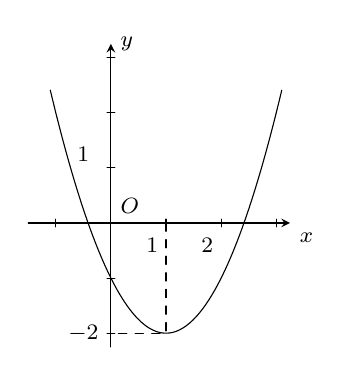
\begin{tikzpicture}[line cap=round,line join=round,font=\footnotesize,>=stealth,scale=0.7]
				\tikzset{label  style/.style={font=\footnotesize}}
				 \draw[->] (-1.5,0)--(3.25,0) node[below right] {$x$};
				\draw[->] (0,-2.25)--(0,3.25) node[right]  {$y$};
				\node  (0,0) [above right]{$O$};
				 \foreach \x in {-1,1,2,3}
				\draw[shift={(\x,0)},color=black]  (0pt,2pt)--(0pt,-2pt);
				\node  at (.75,-0.4) {$1$};
				 \node at (1.75,-0.4) {$2$};
				\foreach \y in {-2,-1,1,2,3} 
				\draw[shift={(0,\y)},color=black] (2pt,0pt)--(-2pt,0pt); 
				\node at  (-0.5,1.25) {$1$};
				\node at  (-0.5,-2) {$-2$};
				\draw[dashed](1,0)--(1,-2)--(0,-2); 
				 \draw [domain=-1.1:3.1,samples=100] plot (\x,{(\x)*(\x)-2*(\x)-1});
			\end{tikzpicture}
		} 
	 \loigiai{
		Đồ thị cắt trục $Oy$ tại điểm có tung độ bằng $-1\Rightarrow c=-1$. Suy ra $y=ax^2+bx-1$.\\ 
		Đồ thị nhận $I\left(1;-2\right)$  làm đỉnh nên $\heva{&\dfrac{-b}{2a}=1\\ &-2=a\cdot 1^2+b\cdot 1-1}\Leftrightarrow\heva{&2a+b=0\\ &a+b=-1}\Leftrightarrow\heva{&a=1\\ &b=-2}$.\\
		 Vậy $y=x^2-2x-1$.
		\begin{itemchoice}
			\itemch Hàm số đã cho có dạng $y=x^2-2x-1$ đúng. 
			\itemch Phương trình  $f(x)=-2$ có đúng hai nghiệm thực phân biệt sai.
			\itemch  Hàm số đã cho đồng biến trên $(1;+\infty)$ đúng.
			\itemch Giá trị lớn nhất của hàm số là $-2$  sai.
		\end{itemchoice}
	} 
\end{ex}


%%%%%%%%%%%%%%%% TRẢ LỜI NGẮN %%%%%%%%%%%%%%%%

% nguồn: MaHoaNH_TraLoiNgan_Lop10
\begin{bt}%[0D3V2-1]%[ma:b89eae95]
	Cho $(\mathrm{P})\colon y=a x^2+b x+c$. Biết đồ thị thỏa đi qua $A(0; 1), B(1; 2), C(3;-1)$. Tính $S = a + b + c$. 
	\shortans{2} 
	\loigiai{ 
		Theo yêu cầu bài toán ta có  hệ phương trình:
		$$\heva{&0 ^ { 2 } \cdot a + 0  \cdot b + c = 1\\& 1 ^ { 2 } \cdot a + 1 \cdot b + c = 2\\&3 ^ { 2 } \cdot a + 3 \cdot b + c = - 1}\Leftrightarrow \heva{&c = 1\\&a + b + c = 2\\&9 a + 3 b + c = - 1}\Leftrightarrow \heva{&a=-\frac{5}{6}\\&b=\frac{11}{6}\\&c=1.}$$
		Vậy $S = a + b + c  = 2$.
	 }
\end{bt}

% nguồn: MaHoaNH_TraLoiNgan_Lop10
\begin{bt}%[0D3V2-1]%[ma:21b92140]
	Cho hàm số bậc  hai có đồ thị là parabol $(P)\colon y=a x^2-4 x+c$ có đỉnh là $I(-2;-1)$. Tính $a+c$.
	\shortans{-6} 
	\loigiai{ 
		Do $(P)$ có đỉnh $I(-2;-1)$ nên 
		 $$\heva{&\dfrac{4}{2 a}=-2\\&a \cdot(-2)^2-4(-2)+c=-1}\Leftrightarrow \heva{&a=-1\\&c=-5.}$$
		Vậy hàm số  bậc hai được xác định là $y=-x^2-4 x-5$. \\
		 Do đó $a+c = -6$.
	 }
\end{bt}

% nguồn: MaHoaNH_TraLoiNgan_Lop10
\begin{bt}%[0D3V2-1]%[ma:98ea0e5d]
	\immini[thm]{ 
	 Cho hàm số bậc hai $y=ax^2+bx+c$ có đồ thị hình bên. Tính $a+100b+c$.
	}{ 
	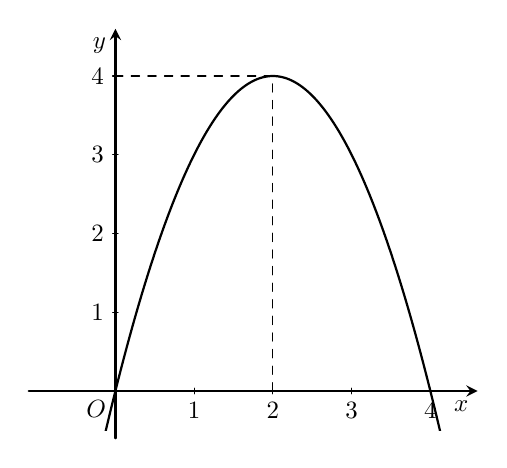
\begin{tikzpicture}[line join=round,line cap=round,>=stealth,thick]
			 \tikzset{every node/.style={scale=0.9}}
			\draw[->] (-1.1,0)--(4.6,0)  node[below left] {$x$};
			\draw[->]  (0,-0.6)--(0,4.6) node[below left] {$y$};
			\draw  (0,0) node [below left] {$O$};
			 \foreach \x/\nx in {1/1,2/2,3/3,4/4}
			\draw[thin]  (\x,1pt)--(\x,-1pt) node [below] {$\nx$};
			\foreach \y/\ny  in {1/1,2/2,3/3,4/4}
			\draw[thin] (1pt,\y)--(-1pt,\y) node [left] {$\ny$}; 
			\draw[dashed,thin](2,0)--(2,4)--(0,4); 
			\begin{scope}
				\clip  (-1,-0.5) rectangle (4.5,4.5);
				 \draw[samples=200,domain=-1:4.5,smooth,variable=\x] plot (\x,{-1*(\x)^2+4*(\x)+0});
			\end{scope}
		\end{tikzpicture}
	} 
	\shortans{399} 
	 \loigiai{
		Đồ thị là một parabol nên hàm số  có dạng $y=a x^2+b x+c$. Ta thấy đồ thị đi qua các điểm $(0; 0),(2; 4)$ và $(4; 0)$ nên ta có
		$$\heva{&c = 0\\&4 a + 2 b + c = 4\\&1 6 a + 4 b +  c = 0}\Leftrightarrow\heva{&a=-1\\&b=4\\&c=0.}$$
		Vậy $a+100b+c  = -1 + 100\cdot 4+0=399$.
	} 
\end{bt}
